
\chapter{Introduction}
\label{chap:introduction}

\begin{quote}
    "We don't tell [computers] what to do, we give them examples... The problem is, sometimes we don't understand how it figured it out."\\ % <--- FORCED NEW LINE HERE
    \vspace{0.5em} % Adds a slightly larger vertical space after the quote text
    \hfill -- Jeff Dean, Head of Google AI \cite{Dean2017BlackBox}
\end{quote}

The prevalence of neural networks (NNs) has established them as a foundational technology in modern artificial intelligence. However, as their use has expanded, so too has attention to their inherent mechanistic limitations. Two major drawbacks of NNs are their lack of explainability—the “black-box” effect—and the substantial computational cost of training. With platforms like Hugging Face and GitHub hosting over one million pre-trained models \cite{huggingface2024review}, interest in addressing these limitations has intensified. Motivated by this vast availability of models, a novel research direction—\textbf{weight space learning}—has emerged as a promising approach to better understand these limitations.

Formally, the weight space of a neural network refers to the set of all possible configurations of its parameters \( W \in \mathbb{R}^n \), where \( n \) is the total number of trainable weights. Each point in this space represents a unique model with a distinct mapping from inputs to outputs. Weight space learning thus concerns learning representations or distributions over this space, capturing how variations in \( W \) relate to model behaviour and how variations in model training influence \( W \). The field generally considers two types of tasks: discriminative and generative.

In discriminative applications, models use the weights of pre-trained networks—often collected into a model zoo \cite{schurholt2022modelzoosdatasetdiverse}—as input to predict meta-information about the original models \cite{unterthiner2021predictingneuralnetworkaccuracy}. The quality of a weight space representation is typically evaluated by the performance of a simple multi-layer perceptron (MLP) in predicting such meta-information, conditioned only on the model's weight embedding.

Common meta-information metrics include the model's final performance and its generalisation gap (the difference between training and validation loss). \cite{salama2024datasetsizerecoverylora} demonstrated that weight embeddings can encode key training characteristics, such as recovering the size of the dataset used for training. These discriminative tasks serve both to validate the quality of the derived weight representations and to provide practical predictive value.

In generative applications, researchers aim to model the underlying distribution of neural network weights \( W \), conditioned on additional information or reference models, \( P(W \mid \dots) \). Sampling from this distribution enables the generation of entirely new model weights.

\cite{schurholt2022hyperrepresentationsgenerativemodelssampling} used an autoencoder with a bottleneck layer to generate hyper-representations of multiple model zoos. Building on this idea, \cite{pmlr-v235-schurholt24a} introduced the Sequential Autoencoder for Neural Embeddings (SANE), which improved scalability and enabled work on much larger models.

To model \( P(W \mid \mathcal{D}) \), \cite{bedionita2025instructionguidedautoregressiveneuralnetwork} employed a Vector Quantised Variational Autoencoder (VQ-VAE), which incorporates dataset information when learning latent weight representations. Similarly, \cite{meynent2025structureenoughleveragingbehavior} modelled \( P(W \mid R) \) by incorporating behavioural differences between reconstructed and original models into the embedding learning process.

While existing weight space learning methods have made significant progress, they typically address isolated aspects of the learning process. Current approaches model either \( P(W \mid \mathcal{D}) \) or \( P(W \mid R) \), but rarely both simultaneously. This is a key limitation: in practice, a model's weights are influenced by both the data it was trained on and the results it achieved. Understanding the joint relationship \( P(W \mid \mathcal{D}, R) \) is essential for explaining model behaviour and for generating models with desired characteristics.

Contrastive learning has emerged as a powerful paradigm for learning unified representations across modalities, as demonstrated by models such as CLIP \cite{radford2021learningtransferablevisualmodels}, which bridge vision and language. A contrastive objective pulls related samples closer in representation space while pushing unrelated samples apart, forming a meaningful joint embedding space for heterogeneous data types. This property makes contrastive learning particularly suitable for modelling the complex distribution \( P(W \mid \mathcal{D}, R) \) --- encompassing visual datasets, high-dimensional weight tensors, and performance metrics --- without requiring a shared native representation.

\begin{figure}[!t]
    \centering
    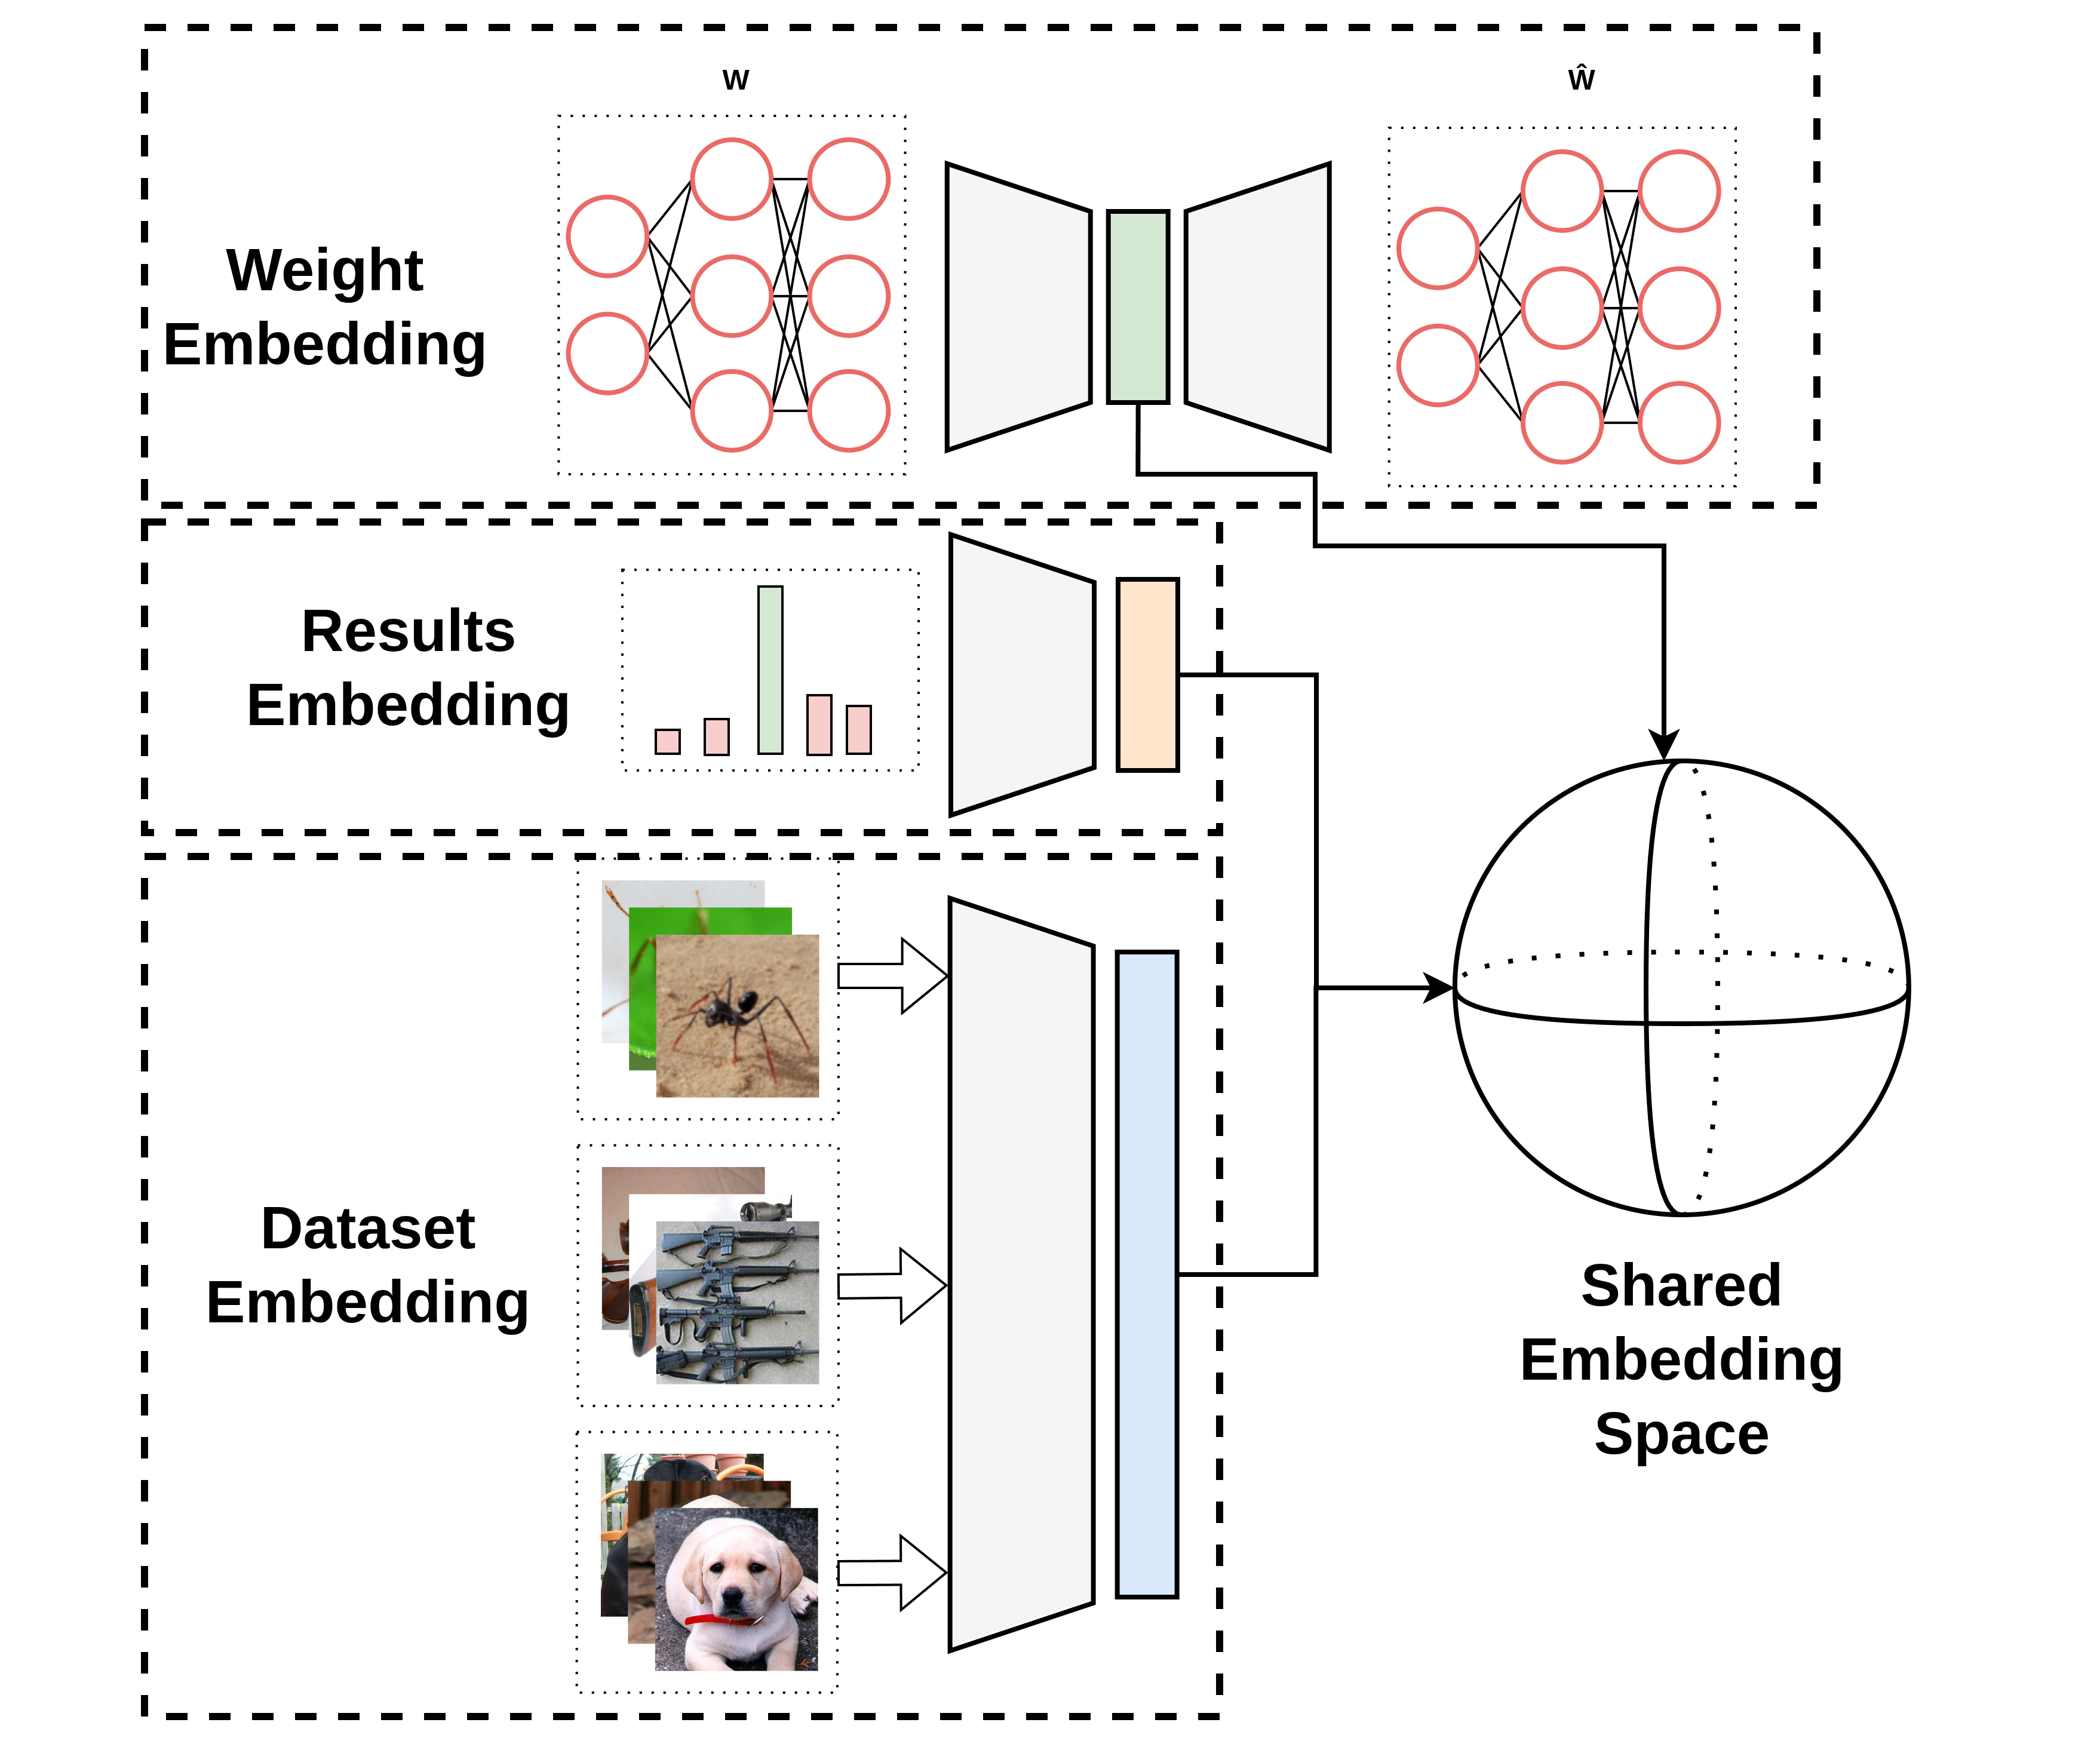
\includegraphics[width=0.75\linewidth]{pipeline.png}
    \caption[The full pipeline of embedding a dataset, model weights and results in a shared embedding space.]{The full pipeline of embedding a dataset, model weights and results in a shared embedding space. }
    \label{fig:pipeline}
\end{figure}

In this report, we develop a contrastive learning framework to create a unified embedding space that jointly represents neural network weights \( W \), the datasets they were trained on \( \mathcal{D} \), and their resulting performance characteristics \( R \). Specifically, we construct two separate encoders—one for dataset embeddings using pre-trained CLIP features, and another for weight embeddings using an autoencoder architecture—alongside a binned result embedding table. These encoders are trained using the contrastive objective NT-Xent \cite{agren2022ntxentlossupperbound}, which encourages related triplets \( (\mathcal{D}, W, R) \) to be close in the shared latent space. Figure \ref{fig:pipeline} depicts a high-level view of the full embedding pipeline.
\newpage

Our central \textbf{hypothesis} is that this unified representation space will enable two key capabilities:

\begin{itemize}
    \item \textbf{Interpretability and Analysis:} Examining geometric relationships within the shared embedding space can reveal how dataset characteristics shape learned weights and model behaviour.
    \item \textbf{Conditional Model Sampling:} The learned distribution enables sampling of model weights conditioned on both dataset properties and target performance metrics--approximating \( P(W \mid \mathcal{D}, R) \).
\end{itemize}

\textbf{Primary Goal}: The primary goal of this report is to demonstrate the viability of our methodology through the success of \textbf{Conditional Model Sampling.} While our hypothesis includes both Interpretability and Conditional Model Sampling, success in the latter strongly suggests a meaningful foundation for the former. Specifically, the ability to accurately sample weights that achieve target performance metrics conditioned on specific dataset ($\mathcal{D}$) and result ($R$) targets confirms that the unified embedding space has meaningfully captured the joint influence of $\mathcal{D}$ and $R$ on the model weights $W$. We will therefore focus on generating meaningful representations, measuring their quality, and critically, performing various forms of conditional model sampling to determine the viability of this specific methodology for generative weight space representations.

The remainder of this report is structured as follows. In Chapter \ref{chap:background}, we discuss the necessary background on weight space learning and contrastive learning. Chapter \ref{chap:method} details the methodology, covering the encoders for $\mathcal{D}$, $W$, and $R$, and the shared contrastive method. Chapter \ref{chap:results} presents our experimental results, focusing on the quality of the learned representations and the core objective of conditional model sampling. Finally, Chapter \ref{chap:conclusion} concludes the report and suggests directions for future work.
